\begin{center}
\Large
\textbf{Геометрический разнобой. 9 июля. }
\end{center}  

\bigskip

\q1. а) Докажите, что на первом рисунке площадь закрашенной части равна площади незакраменной.


б) Докажите, что на втором рисунке площадь закрашенной дважды части равна площади незакрашенной совсем.

\begin{center}

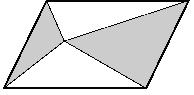
\includegraphics[width=0.4\textwidth]{2b.JPG}
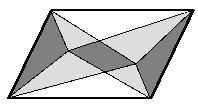
\includegraphics[width=0.4\textwidth]{2d.JPG}
\end{center}

% Про лемму о линолеуме

\q2. На сторонах $AB$, $BC$ и $CA$ треугольника $ABC$, площадь которого равна $S$, выбраны точки $C_1$, $A_1$ и $B_1$ так, что $AC_1 = 2C_1B$, $BA_1=2A_1C$ и $CB_1=2B_1A$. Чему равна площадь треугольника $A_1B_1C_1$? 

% на площадь и отношение оснований

\q3. Дан равносторонний треугольник $ABC$ и точка $X$ внутри. Докажите, что сумма расстояний от точки $X$ до сторон треугольника не зависит от точки $X$
% на площадь

\q4т. а) На сторонах прямоугольного треугольника во внешнюю сторону построены квадраты. Докажите, что площади тёмных треугольничков на рисунке равны.\\

\begin{center}
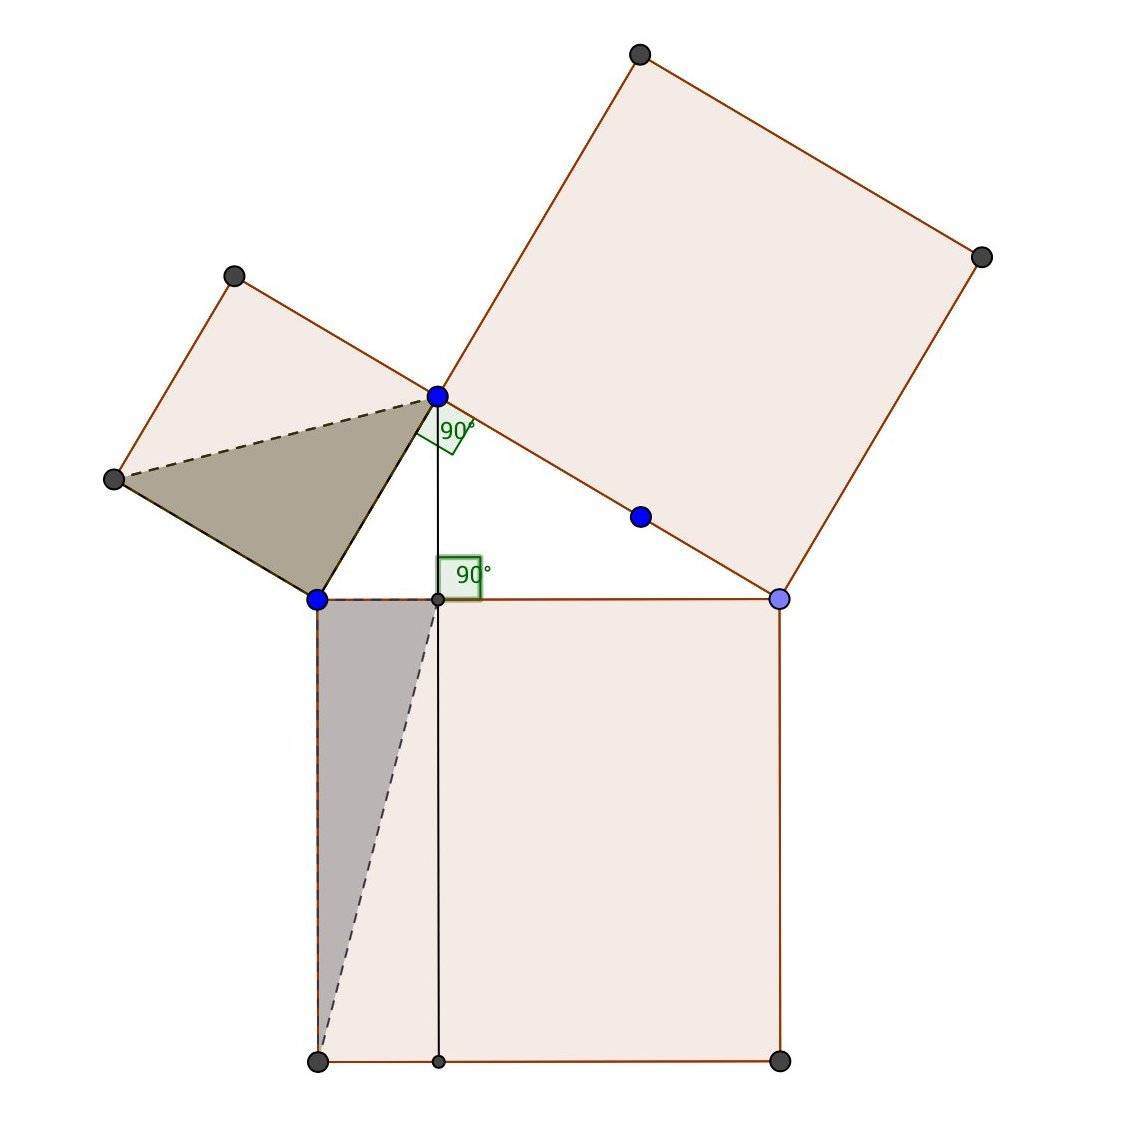
\includegraphics[width=0.4\textwidth]{pifagor.jpg}
\end{center} 


б) Выведите отсюда теорему Пифагора.

%Теорема Пифагора 


\q5т. а) Диагонали четырёхугольника $ABCD$ перпендикулярны. Докажите, что $AB^2+CD^2=AD^2+BC^2$.


б) Докажите, что если в четырёхугольнике $ABCD$ выполнено $AB^2+CD^2=AD^2+BC^2$, то его диагонали перпендикулярны. 
%На теорему Пифагора


\q6т. Треугольники~$ABC$ и~$A_1B_1C_1$ таковы, что $AB=A_1B_1$,
\quad $BC=B_1C_1$
и~$\angle A = \angle A_1$. Докажите, что либо эти треугольники равны, либо
$\angle C + \angle C_1 = 180^{\circ}$.
% четвёртый признак

\q7. На гипотенузе~$AC$ прямоугольного треугольника $ABC$ выбрали точку~$D$
такую, что $BC=CD$. На катете~$BC$ выбрали такую точку~$E$, что $DE=CE$.
Докажите, что $AD+BE=DE$.
% На равенство треугольников с доп построением


\q8.  В треугольнике $ABC$ \quad $AB<AC$. Прямая, проходящая через вершину~$B$ параллельно~$AC$, пересекает
биссектрису внешнего угла~$A$ в точке~$D$. Прямая, проходящая через вершину~$C$ параллельно~$AB$, пересекает
эту биссектрису в точке~$E$. На стороне~$AC$ выбрана точка~$F$ так, что $FC=AB$.  Доказать, что $DF=FE$.

% На равенство треугольников с доп построением


\q9. Внутри треугольника $ABC$ отмечена точка $M$, так что при этом
$\angle  BAM=\angle ABC$, $\angle AMB=100^{\circ}$,
$\angle ACB=70^\circ$. Докажите, что $BM<AC$.
